\chapter{Experiments and Results}
\label{ch:results}
The performance of the proposed approach is tested on two publicly available datasets: EgoGesture egocentric hand gesture recognition, and  NVIDIA Dynamic Hand Gesture dataset. In evaluation process, equidistant frames of different size are used, and these frames are slided 1 frame at each iteration.\\

\section{Offline Results Using EgoGesture Dataset}
\begin{table}[b!]
    \centering
    \begin{tabular}{ccc}
        \specialrule{.1em}{.5em}{.5em}
        \multicolumn{1}{c}{\multirow{2}{*}{\textbf{Model}}} & \multicolumn{1}{c}{\multirow{2}{*}{\textbf{Input}}} & \multicolumn{1}{c}{\textbf{Modality}}                                   \\ \cline{3-3} \addlinespace
        \multicolumn{1}{c}{}                       & \multicolumn{1}{c}{}                       & \multicolumn{1}{c}{\textbf{RGB}}\\
        \specialrule{.1em}{.3em}{.3em}
        C3D             & 16-frames     & 82.01   \\ 
        C3D             & 24-frames     & 87.85 \\ 
        C3D             & 32-frames     & 94.14  \\ 
        \specialrule{.1em}{.3em}{.3em}
        ResNeXt-101     & 32-frames     &  95.72 \\ 
        \specialrule{.1em}{.5em}{.5em}
    \end{tabular}
    \caption{Results of Pretrained models on the Jester dataset.}
	\label{tab:jester_classifier}
\end{table}
EgoGesture dataset is a recent multi-modal large scale dataset for egocentric hand gesture recognition \cite{zhang_egogesture:_2018}. This dataset is created not only for segmented gesture classification, but also for gesture detection in continuous data. There are 83 classes of static or dynamic gestures collected from 6 diverse indoor and outdoor scenes. The dataset contains 2,081 RGB-D videos having 24,161 gesture samples from 50 distinct subjects. The dataset splits are created by distinct subjects with ratio 3:1:1 resulting in 1,239 training, 411 validation and 431 testing videos, having 14416, 4768 and 4977 gesture samples as suggested in \cite{zhang_egogesture:_2018}, respectively. All models are first pretrained on Jester dataset \cite{jester}, and results for these pretrained models are shown in Table \ref{tab:jester_classifier}. For test set evaluations, we have used both training and validation set for training.\\

We initially investigated the performance of C3D and ResNeXt architectures on the offline classification task. Table \ref{tab:egogesture_benchmark} shows the comparison of used architectures with the state-of-the-art architectures. ResNeXt-101 architecture with 32-frames input achieves the best performance. Moreover, all RGB-D modalities in Table \ref{tab:egogesture_benchmark}, except for our architectures, apply late fusion which is unpractical for real-time applications. We have used data level fusion for RGB-D modality as proposed in \cite{kopuklu2018motion}.\\

\begin{table}[t!]
    \centering
    \begin{tabular}{ccccc}
        \specialrule{.1em}{.5em}{.5em}
        \multicolumn{1}{c}{\multirow{2}{*}{\textbf{Model}}} & \multicolumn{1}{c}{\multirow{2}{*}{\textbf{Input}}} & \multicolumn{3}{c}{\textbf{Modality}}                                   \\ \cline{3-5} \addlinespace
        \multicolumn{1}{c}{}                       & \multicolumn{1}{c}{}                       & \multicolumn{1}{c}{\textbf{RGB}} & \multicolumn{1}{c}{\textbf{Dept}h} & \textbf{RGB-D} \\
        \specialrule{.1em}{.3em}{.3em}
        C3D             & 16-frames     & 86.88          & 88.45                    & 89.45    \\ 
        C3D             & 24-frames     & 89.20          & 89.07                    & 91.22    \\ 
        C3D             & 32-frames     & 83.32          & 91.44                    & \textbf{91.80}    \\ 
        \specialrule{.1em}{.3em}{.3em}
        ResNeXt-101     & 16-frames     & 90.94          & 91.80                    & 91.82    \\ 
        ResNeXt-101     & 24-frames     & 92.89          & 93.47                    & 93.73   \\ 
        ResNeXt-101     & 32-frames     & 93.75          & \phantom{\textbf{*}}\textbf{94.03}\textbf{*}           & 93.93             \\ 
        \specialrule{.1em}{.5em}{.5em}
    \end{tabular}
    \caption{Classifier's classification results on the test set of \textbf{EgoGesture} dataset.}
	\label{tab:egogesture_classifier}
\end{table}
\begin{table}[t!]
    \centering
    \begin{tabular}{ccccc}
        \specialrule{.1em}{.5em}{.5em}
        \multicolumn{1}{c}{\multirow{2}{*}{\textbf{Model}}} & \multicolumn{1}{c}{\multirow{2}{*}{\textbf{Input}}} & \multicolumn{3}{c}{\textbf{Modality}}                                   \\ \cline{3-5} \addlinespace
        \multicolumn{1}{c}{}                       & \multicolumn{1}{c}{}                       & \multicolumn{1}{c}{\textbf{RGB}} & \multicolumn{1}{c}{\textbf{Dept}h} & \textbf{RGB-D} \\
        \specialrule{.1em}{.3em}{.3em}
        ResNet-10     & 8-frames      & 96.58          & \phantom{\textbf{*}}99.39\textbf{*}           & 98.78    \\ 
        ResNet-10     & 16-frames     & 97.00          & 99.64           & 99.17    \\ 
        ResNet-10     & 24-frames     & 97.13          & 99.15                    & 99.28    \\ 
        ResNet-10     & 32-frames     & 96.65          & \textbf{99.68}           & 99.61    \\ 
        \specialrule{.1em}{.3em}{.3em}
    \end{tabular}
    \caption{Detector's classification results on the test set of \textbf{EgoGesture} dataset.}
	\label{tab:egogesture_detector}
\end{table}
\begin{table}[b!]
	\centering
	\begin{tabular}{lccc}
		\specialrule{.1em}{.5em}{.5em}
		\textbf{Modality} & \textbf{Recall} & \textbf{Precision} & \textbf{f1-score}  \\ 
		\specialrule{.1em}{.3em}{.3em}
		RGB            & 96.64	    & 97.10     & 96.87   \\
		Depth          & 99.37		& 99.43		& \textbf{99.40}   \\
		RGB-D          & 98.80		& 98.97		& 98.88   \\
		\specialrule{.1em}{.3em}{.3em}
	\end{tabular}
	\caption{Detection results on the test set of \textbf{EgoGesture} dataset.}
	\label{tab:egogesture_det}
\end{table}

Secondly, we investigated the effects of the number of input frames on the gesture detection and classification performance. Results in Table \ref{tab:egogesture_detector} and Table\ref{tab:egogesture_classifier} shows that we achieve a better performance as we increase the input size, for all the modalities. This situation is highly dependent on the characteristics of the used datasets, especially on the average sample duration of gestures that is 38.4 frames for EgoGesture dataset as shown in Figure \ref{fig:weight} (b).\\ 
\begin{figure}[b!]%
\centering
\subfigure[]{%
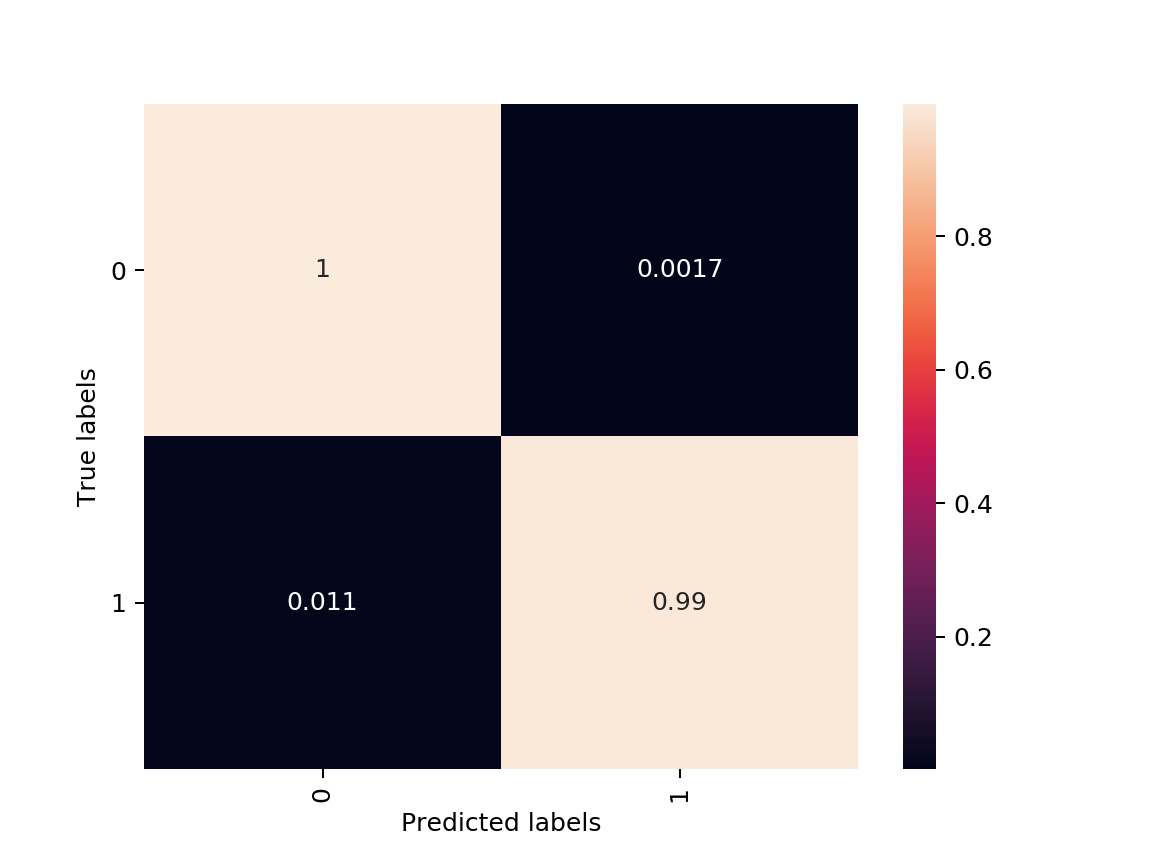
\includegraphics[width =0.45 \linewidth]{figures/egogesture_confusion_matrix}}%
\label{fig:staego}%
\qquad
\subfigure[]{%
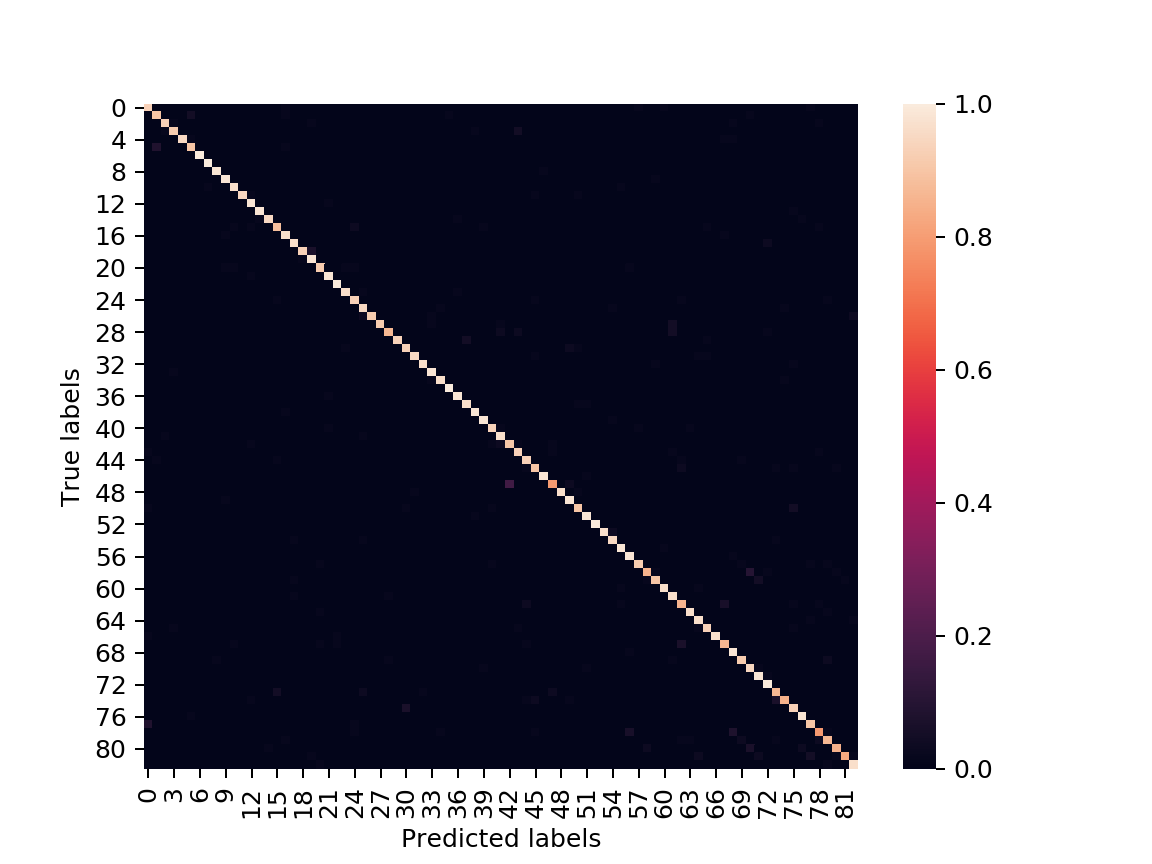
\includegraphics[width = 0.45 \linewidth]{figures/egogesture_confusion_matrix2}}%
\caption{Mormalized confusion matrices for the choosen detector (a) and classifier (b) in \textbf{EgoGesture} dataset.}
\label{fig:egocm}
\end{figure}
\begin{table}[t!]
    \centering
    \begin{tabular}{lcccc}
        \specialrule{.1em}{.5em}{.5em}
        \multicolumn{1}{c}{\multirow{2}{*}{\textbf{Model}}} & \multicolumn{1}{c}{\multirow{2}{*}{\textbf{Input}}} & \multicolumn{3}{c}{\textbf{Modality}}                                   \\ \cline{3-5} \addlinespace
        \multicolumn{1}{c}{}      & \multicolumn{1}{c}{}    & \textbf{RGB} & \textbf{Depth} & \textbf{RGB-D} \\
        \specialrule{.1em}{.3em}{.3em}
        VGG-16 \cite{zhang_egogesture:_2018}          & 16-frames     & 62.50    & 62.30    & 66.50    \\
        VGG-16 + LSTM \cite{zhang_egogesture:_2018}   & 16-frames     & 74.70    & 77.70    & 81.40    \\
        C3D                                           & 16-frames     & 86.88    & 88.45    & 89.45    \\ 
        ResNeXt-101                                   & 16-frames     & 90.94    & 91.80    & 91.82    \\ 
        C3D+LSTM+RSTTM \cite{zhang_egogesture:_2018}  & 16-frames     & 89.30    & 90.60    & 92.20    \\
        \specialrule{.1em}{.3em}{.3em}
        ResNeXt-101     & 32-frames     & 93.75          & \textbf{94.03}           & 93.93             \\ 
        \specialrule{.1em}{.5em}{.5em}
    \end{tabular}
    \caption{Comparison with state-of-the-art on the test set of EgoGesture dataset.}
	\label{tab:nv_benchmark}
\end{table}

Thirdly, the modalities (RGB, Depth and RGB-D) are investigated through fixing window-size of input frames. We can see that the models with RGB-D and Depth modalities always show better performance than the models with RGB. Because Depth sensor filters out background motion, and it allow models to focus more on the hand motion, and learn discriminative features better. Additionally, The state-of-the-art accuracies in classification task of EgoGesture datasets are shown in Table \ref{tab:egogesture_benchmark}. We can clearly say that ResNet-101 architecture with 32-frames of Depth modality outperforms the proposed architecture in \cite{zhang_egogesture:_2018}.  \\

After offline classification results, we decided to use ResNet-10 with window of size 8 and Depth images as our detector even though the ones with 24-frames and 32-frames have higher accuracy rate. This is because having smaller window size allows the detector to be more robust in detection of the start and the end of gestures. Moreover, It is very critical that we do to miss any gestures, and this is highly dependent on the detector's recall rate. The detailed results of this model is shown in Table \ref{tab:egogesture_det}. \\

Finally, we investigated the performance of the detector (ResNet-10 with window size of 8 and trained on Depth images) and the classifier (ResNext-101 with window size of 32 and trained on Depth images) with confusion matrix shown in Figure \ref{fig:egocm}.\\
\clearpage
\section{Offline Results Using nvGesture Dataset}
\begin{table}[h!]
    \centering
    \begin{tabular}{ccccc}
        \specialrule{.1em}{.5em}{.5em}
        \multicolumn{1}{c}{\multirow{2}{*}{\textbf{Model}}} & \multicolumn{1}{c}{\multirow{2}{*}{\textbf{Input}}} & \multicolumn{3}{c}{\textbf{Modality}}                                   \\ \cline{3-5} \addlinespace
        \multicolumn{1}{c}{}                       & \multicolumn{1}{c}{}                       & \multicolumn{1}{c}{\textbf{RGB}} & \multicolumn{1}{c}{\textbf{Dept}h} & \textbf{RGB-D} \\
        \specialrule{.1em}{.3em}{.3em}
        C3D             & 16-frames     & 62.67          & 70.33           & 64.10             \\ 
        C3D             & 24-frames     & 65.35          & 70.33           & 66.40             \\ 
        C3D             & 32-frames     & 73.86          & \textbf{77.18}           & 72.61             \\ 
        \specialrule{.1em}{.3em}{.3em}
        ResNeXt-101     & 16-frames     & 66.40          & 72.82                    & 74.65    \\ 
        ResNeXt-101     & 24-frames     & 72.40          & 79.25          & 75.31             \\ 
        ResNeXt-101     & 32-frames     & 78.63          & \phantom{\textbf{*}}\textbf{83.82}\textbf{*}           & 79.67             \\ 
        \specialrule{.1em}{.5em}{.5em}
    \end{tabular}
    \caption{Classifier's classification results on the test set of \textbf{nvGesture} dataset.}
	\label{tab:nvgesture_classifier}
\end{table}
\begin{table}[h!]
    \centering
    \begin{tabular}{ccccc}
        \specialrule{.1em}{.5em}{.5em}
        \multicolumn{1}{c}{\multirow{2}{*}{\textbf{Model}}} & \multicolumn{1}{c}{\multirow{2}{*}{\textbf{Input}}} & \multicolumn{3}{c}{\textbf{Modality}}                                   \\ \cline{3-5} \addlinespace
        \multicolumn{1}{c}{}                       & \multicolumn{1}{c}{}                       & \multicolumn{1}{c}{\textbf{RGB}} & \multicolumn{1}{c}{\textbf{Dept}h} & \textbf{RGB-D} \\
        \specialrule{.1em}{.3em}{.3em}
        ResNet-10     & 8-frames      & 70.22          &  \phantom{\textbf{}} 97.30\textbf{*}        & 93.15    \\ 
        ResNet-10     & 16-frames     & 85.90          & 97.82           & 94.81    \\ 
        ResNet-10     & 24-frames     & 89.00          & \textbf{98.02}           & 97.30    \\ 
        ResNet-10     & 32-frames     & 93.88         & 97.30            & 95.33    \\ 
        \specialrule{.1em}{.3em}{.3em}
    \end{tabular}
    \caption{Detector's classification results on the test set of \textbf{nvGesture} dataset.}
	\label{tab:nvgesture_detector}
\end{table}
In nvGesture dataset, we followed similar validation procedure to EgoGesture dataset except that nvGesture dataset does not have a validation set so we trained our models for fixed number of epochs (30) and used the last one as our reference.\\ 
\begin{table}[b!]
	\centering
	\begin{tabular}{lccc}
		\specialrule{.1em}{.5em}{.5em}
		\textbf{Modality} & \textbf{Recall} & \textbf{Precision} & \textbf{f1-score}  \\ 
		\specialrule{.1em}{.3em}{.3em}
		RGB            & 70.22	    & 80.31     & 74.93  \\
		Depth          & 97.30		& 97.41		& \textbf{97.35}   \\
		RGB-D          & 93.15		& 93.31		& 93.23 \\
		\specialrule{.1em}{.3em}{.3em}
	\end{tabular}
	\caption{Detection results on the test set of \textbf{nvGesture} dataset.}
	\label{tab:nvgesture_det}
\end{table}

Performance of the detector and the classifier architectures can be seen in Table \ref{tab:nvgesture_detector} and Table \ref{tab:nvgesture_classifier}, respectively. These results confirm our implications in EgoGesture dataset as models with Depth and RGB-D modalities shows better performance than models with RGB. Also In nvGesture dataset, duration of every gesture corresponds to exactly 81 frames. Consequently, the more window-size of model the higher accuracy rate as it is the case in EgoGesture dataset as well. \\

Additionally, Table \ref{tab:nvgesture_classifier} shows comparision betwenn the state-of-the-art models and our classifer architectures. ResNet-101 with 32 frames showed comparable results with R3DCNN \cite{molchanov_online_2016}. Similarly, the confusion matrices for the selected detector and classifier on nvGesture dataset can be seen in Figure \ref{fig:nvcm}.\\
\begin{figure}[h!]%
\centering
\subfigure[]{%
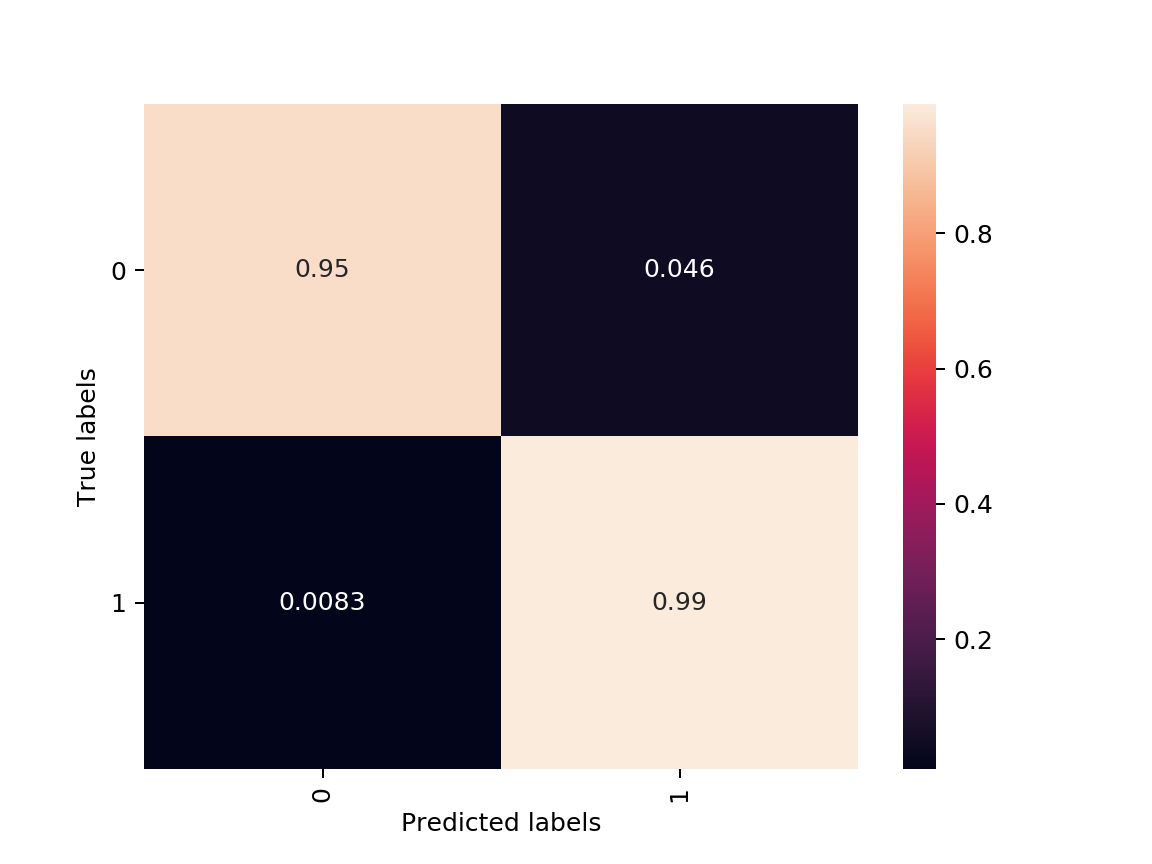
\includegraphics[width =0.45 \linewidth]{figures/nv_confusion_matrix}}%
\label{fig:staego}%
\qquad
\subfigure[]{%
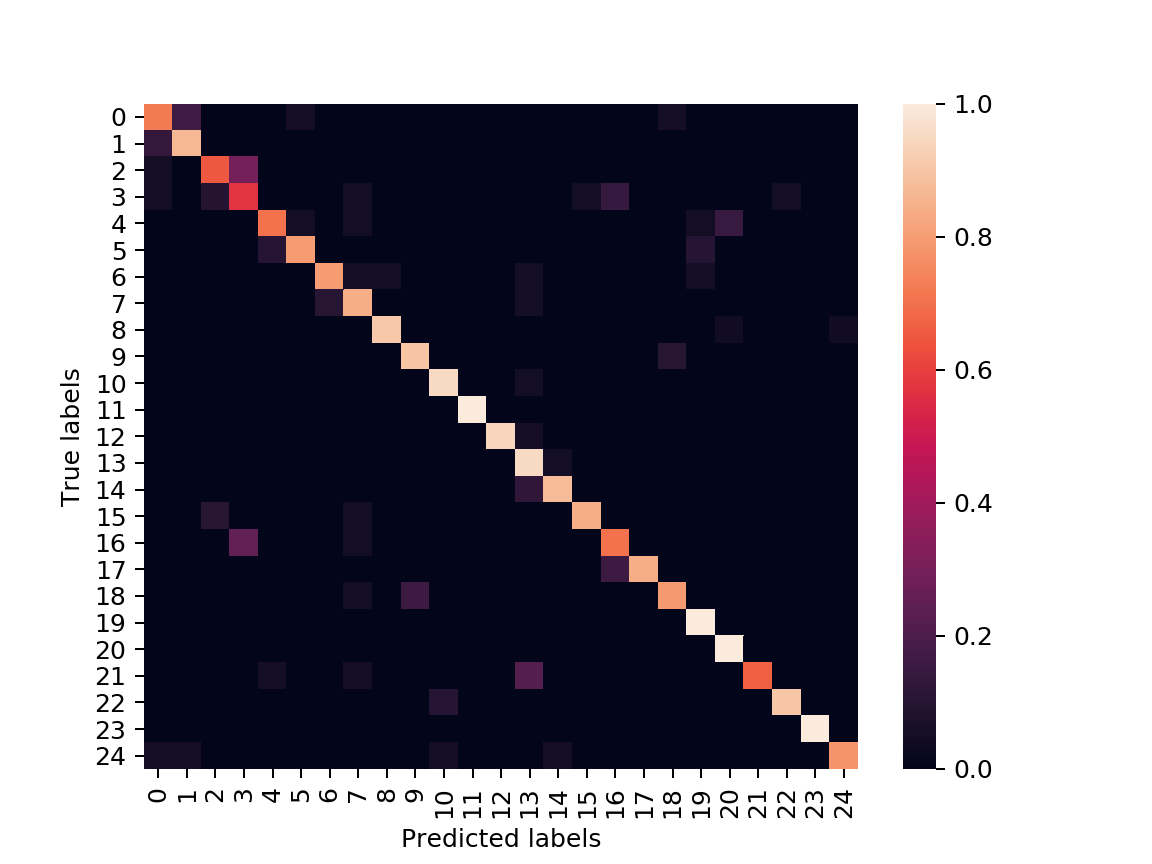
\includegraphics[width = 0.45 \linewidth]{figures/nv_confusion_matrix2}}%
\caption{Normalized confusion matrices for the chosen detector (a) and classifier (b) in \textbf{nvGesture} dataset.}
\label{fig:nvcm}
\end{figure}

\begin{table}[t!]
    \centering
    \begin{tabular}{lccccc}
        \specialrule{.1em}{.5em}{.5em}
        \multicolumn{1}{c}{\multirow{2}{*}{\textbf{Model}}} & \multicolumn{1}{c}{\multirow{2}{*}{\textbf{Input}}} & \multicolumn{4}{c}{\textbf{Modality}}                                   \\ \cline{3-6} \addlinespace
        \multicolumn{1}{c}{}      & \multicolumn{1}{c}{}    & \textbf{RGB} & \textbf{Depth} & \textbf{RGB-D} &   \textbf{RGBD + flow} \\
        \specialrule{.1em}{.3em}{.3em}
        C3D             & 16-frames     & 62.67          & 70.33           & 64.10          & -   \\ 
        R3DCNN \cite{molchanov_online_2016}                          & 16-frames     & 74.10    & 80.30    & -  & 83.8  \\ 
       ResNeXt-101     & 16-frames     & 66.40          & 72.82                    & 74.65   & - \\
        \specialrule{.1em}{.3em}{.3em}
        ResNeXt-101     & 32-frames     & 78.63        & \phantom{\textbf{*}}\textbf{83.82}\textbf{*}           & 79.67        & -       \\ 
        \specialrule{.1em}{.5em}{.5em}
    \end{tabular}
    \caption{Comparison with state-of-the-art on the test set of nvGesture dataset. In \cite{molchanov_online_2016} a proposed architecture with RGB, Depth, optical flow (annotated as "flow" in the Table) modalities achieves state-of-the-art 83.8\% accuracy.}
	\label{tab:egogesture_benchmark}
\end{table}

\clearpage
\section{Real-Time Classification Results}
\begin{figure}[b!]%
\centering
\subfigure[]{%
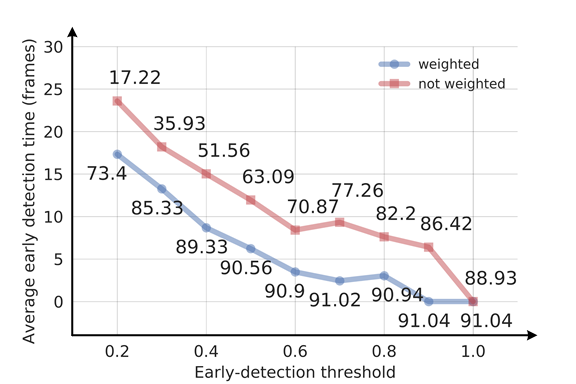
\includegraphics[width =0.6 \linewidth]{figures/egogesture_det}}%
\label{fig:staego}%
\qquad
\subfigure[]{%
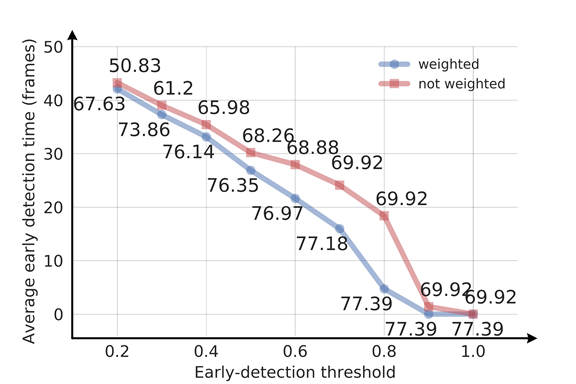
\includegraphics[width = 0.6 \linewidth]{figures/nv_det}}%
\caption{Correctly predicted classes early-detection durations with respect to different thresholds (0.2-1.0) in \textbf{(a) EgoGesture} and  
\textbf{(b) nvGesture} datasets. Numerals on each data point represent the overall Levenshtein accuracies. Blue color refers to the "weighted" approach in single-time activation, and green color refers to "not weigted" approach. In both cases, duration between the end of gesture and detected time decreases as threshold increases, which is expected. Besides that, we can see that the weighted approach increases the Levenshtein accuracies drastically.}
\label{fig:stanv}
\end{figure}
 In online (real-time) evaluation, we selected best performing models in both dataset, which have \textbf{*} sign in corresponding Tables. Egogesture and nvGesture respectively have 431 and 482 video samples in their test set. We evaluated our proposed architecture on each video seperately and calculated an average Levenshtein accuracy at the end. We achieved 91.04\% (in Egogesture ) and 77.39\% (in nvGesture) overall Levenshtein accuracy.\\

Moreover, the early detection times are investigated by simulating different early detection threshold levels ($\tau_{early}$) levels (0.2-1.0). Figure \ref{fig:stanv} compares early detection durations of weigted-averaging and uniformly-averaging approaches for both EgoGesture and nvGesture datasets. As expected, the more the early detection threshold is the later the models detect the gesture. Additionally weighted approach clearly achieves better Levenshtein accuracy rate for the same early-detection threshold levels. This proves that we managed to get rid of the ambiguity at the beginning of gestures by assigning lower weights.\\ 

As a result, it is important to note that, comparison of the Levenshtein metric and offline accuracy is not fair even though there is a strong positive correlation between them. This is because the Levenshtein metric not only evaluate misclassification rate but also multiple prediction rate of the same gesture. Nevertheless, the offline accuracy rate of a model can be also considered as the upper bound for the Levenshtein metric.\\